\section{Traffic Light}

\subsection{Scope}

In this tutorial you will build an example with a more advanced state machine.
To make it more appealing we've added a little GUI with two traffic lights, one for the cars and one for pedestrians.
The GUI also contains a button that can be used to request green for pedestrians.

You will perform the following steps:

\begin{enumerate}
\item create a new model from scratch
\item create a pedestrian light actor
\item perform a first test
\item implement the behavior
\item do some configuration
\end{enumerate}

\subsection{Create a new model from scratch}

The easiest way to create a new \eTrice{} Project is to use the eclipse project wizard. From the eclipse file 
menu select \emph{File->New->Project} and create a new \emph{Empty eTrice Java Project} and name it \textbf{TrafficLight}.

In the model directory locate TrafficLight.room and edit it. We only rename a little.
The model should look like this:

\begin{lstlisting}[language=ROOM]
RoomModel TrafficLight {

	LogicalSystem TrafficLight {
		SubSystemRef main: Main
	}

	SubSystemClass Main {
		ActorRef pedLight: PedestrianLight
		LogicalThread defaultThread
	}

	ActorClass PedestrianLight { }

}
\end{lstlisting}

Since the mapping model references our logical system and sub system we also need to adjust that:

\begin{lstlisting}[language=etmap]
MappingModel TrafficLight {
	import TrafficLight.* from "TrafficLight.room"
	import TrafficLight.* from "TrafficLight.etphys"
	Mapping TrafficLight -> PhysSys1 {
		SubSystemMapping main -> nodeRef1 {
			ThreadMapping defaultThread -> PhysicalThread1
		}
	}
}
\end{lstlisting}

Since we need a timer we have to include the TimingService from the modellib (see \ref{sec:ping_pong_tutorial}).
We have to add an import statement

\begin{lstlisting}[language=ROOM]
import room.basic.service.timing.* from "../../org.eclipse.etrice.modellib.java/model/TimingService.room"
\end{lstlisting}

Then we open the structure of \textit{Main} and add an actor reference \textit{timingSvc} of type \textit{ATimingService}.
The we create a layer connection from \textit{pedLight} to \textit{timingSvc}.

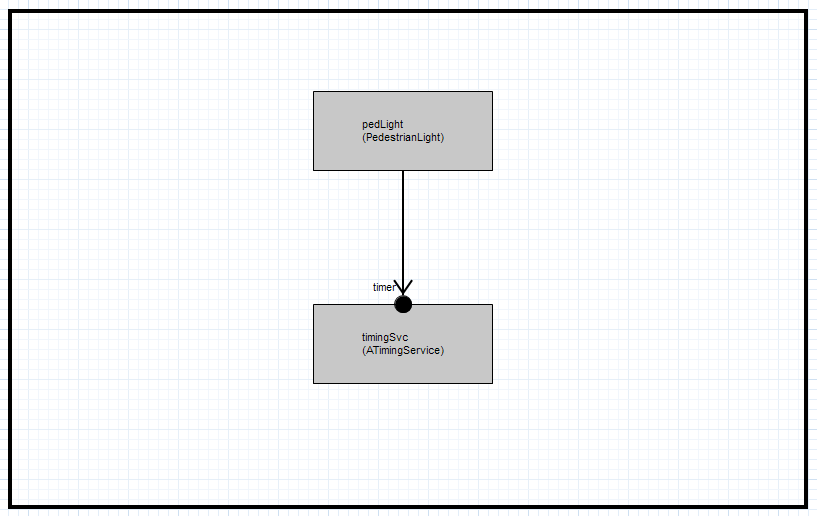
\includegraphics[width=0.6\textwidth]{images/018-timingSvc.png}

Now we are ready to 

\subsection{Implement the \textit{PedestrianLight} Actor}

Since our GUI is connected using TCP/IP sockets we need to add an instance of the \textit{ATcpClient}.
We will explain the simple protocol used to control the GUI later as we go.

Again we first have to add an import statement.

\begin{lstlisting}[language=ROOM]
import room.basic.service.tcp.* from "../../org.eclipse.etrice.modellib.java/model/TcpService.room"
\end{lstlisting}

Then we can add the TCP client as \textit{socketClient}.
As we see the TCP client hast two ports on its interface. One is for controlling the connection, the other one
is used for the data. Therefore we add internal end ports to our actor and connect them
(make sure to add the ports as conjugated):

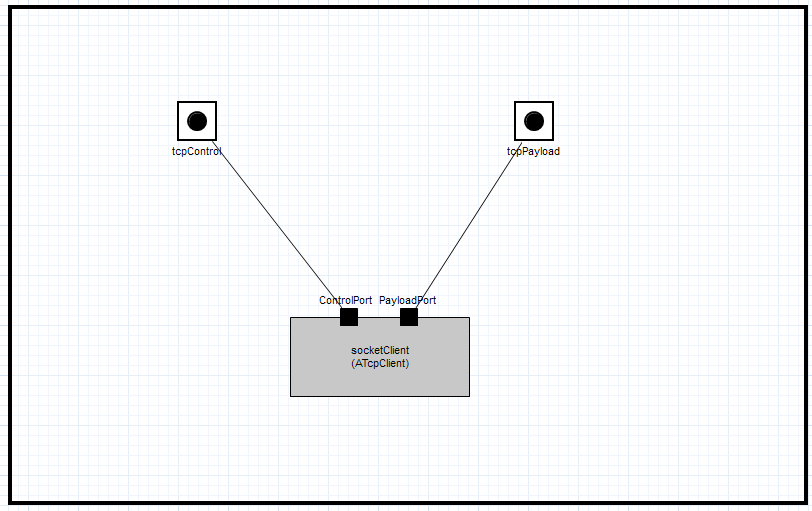
\includegraphics[width=0.6\textwidth]{images/018-socketSvc.png}

Now we can begin to implement the behavior of our actor.
In the initial state we try to connect our GUI application via a socket connection.
So we create a State \textit{OpenSocket} and an initial transition to it.
In the entry code we use the \textit{Messages} button and select \textit{open} for the \textit{tcpControl} port.

The code fragment
\begin{lstlisting}[language=ROOM]
tcpControl.open(data);
\end{lstlisting}
is inserted for us.

(We've already added a semi colon at the end of the statement.)

By inspecting the \textit{PTcpControl} protocol we find that the \textit{open} message takes an argument
of type \textit{DTcpControl} which in turn consists of a string - the IP address - and an integer for the
port number.

So we complete the call to tcpControl.open() by inserting the connection data:
\begin{lstlisting}[language=Java]
tcpControl.open(new DTcpControl("localhost", 4443));
\end{lstlisting}

At this point we can

\subsection{Perform a first test}

First we generate code using the launch configuration \textit{gen\_TrafficLightJava.launch} the wizard created for us.
We observe that the code doesn't compile because we introduced a dependency to the \textit{modellib.java}.
So we add this project to our Java build path.

Now the build should be clean.

Prior to the generated application we have to launch the GUI with the expected socket 4443 that we've configured above.
So we install the 'eTrice Trafficlight for Tutorials' project in our work space using the New Wizard.
Locate the launch configuration \textit{trafficlight\_port\_4443.launch} and run it. A little Window pops up

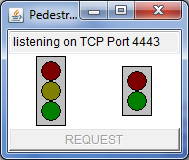
\includegraphics{images/018-trafficlightGUI.png}

which tells us it is listening on socket 4443.

Then we launch our application using \textit{run\_TrafficLight.launch}.
The console window shows

\begin{verbatim}
***   T H E   B E G I N   ***
*** MainComponent /TrafficLight/main::init ***
type 'quit' to exit
Client Init !
\end{verbatim}

and the GUI indicates that it is connected with a client:

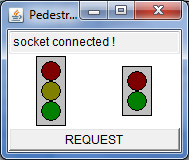
\includegraphics{images/018-trafficlightGUI-connected.png}

After entering 'quit' in the console window we turn back to the behavior of our \textit{PedestrianLight} actor.

\subsection{Implement the \textit{PedestrianLight} Behavior}

The \textit{ATcpClient} returns \textit{established()} if the socket connection is created and ready to use.
So we use this trigger to make a transition into the operational state.

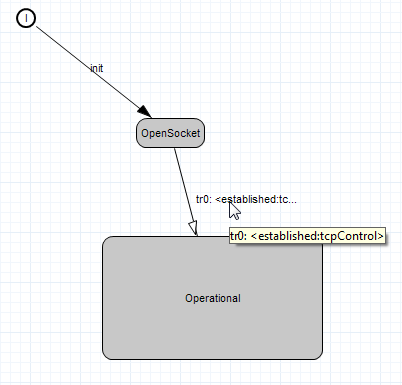
\includegraphics{images/018-trans-to-operational.png}

The switching of the lights will be implemented in a sub graph of the \textit{Operational} state.

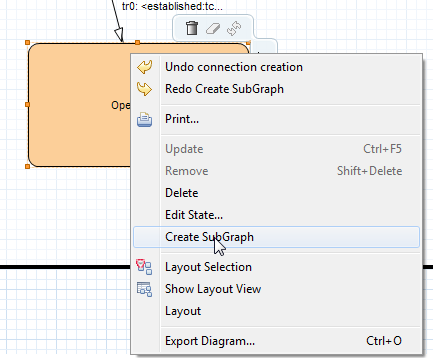
\includegraphics{images/018-create-sub-graph.png}

Now we turn to the sub state machine of \textit{Operational}. We need to cyclically loop through all
phases of the traffic light.

\begin{tabular}{|c|c|c|c|}
\hline 
State & Car Lights & Ped Lights & timeout [s]\\ 
\hline 
AllRed & red & red & 1 \\ 
\hline 
CarGreen & green & red & n/a \\ 
\hline 
CarYellow & yellow & red & 1 \\ 
\hline 
CarRed & red & red & 1 \\ 
\hline 
PedGreen & red & green & 3 \\ 
\hline 
\end{tabular}

\textit{AllRed} will be the initial state. There we start a timeout after which we do the transition
to \textit{CarGreen}. We will stay in this state until the request button is pushed which means that we can trigger
on \textit{recive()} from the \textit{tcpPayload} port. Since nothing else will be sent back from our GUI we don't have
to look at the contents of the payload. The transition ends in \textit{CarYellow} where we again start a timeout
which will take us to the next state and so on until we again reach \textit{CarGreen} which completes the cycle.

The next thing we need is a \textit{SAP} for our timeout. We will call it \textit{'timeout'}.
Then we can create the states and transitions in the sub state machine of \textit{Operational}.

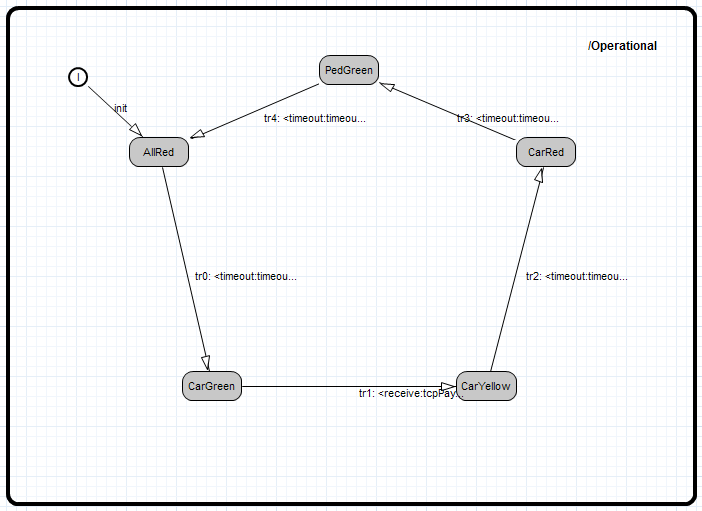
\includegraphics[width=0.9\textwidth]{images/018-operational.png}

The only thing that is left to be done is the actual switching of the lights in our GUI.
We have to send the commands as strings terminated by new line characters.
The GUI reacts on the following commands:

\begin{itemize}
\item "pedLights=red\textbackslash{}n"
\item "pedLights=green\textbackslash{}n"
\item "carLights=red\textbackslash{}n"
\item "carLights=yellow\textbackslash{}n"
\item "carLights=green\textbackslash{}n"
\end{itemize}

To simplify the code we have to add to the entry codes of the states we propose to add two methods:

\begin{lstlisting}[language=ROOM]
Operation sendString(text: string) {
	"tcpPayload.send(new DTcpPayload(1, text.length(), text.getBytes()));"
}
Operation setLights(car: Light, ped: Light) {
	"sendString(\"carLights=\"+getCmd(car)+\"\\n\");"
	"sendString(\"pedLights=\"+getCmd(ped)+\"\\n\");"
}
Operation getCmd(light: Light): string {
	"switch(light) {
	case Light.RED: return \"red\";
	case Light.GREEN: return \"green\";
	case Light.YELLOW: return \"yellow\";
	default: return \"\";
	}"
}
\end{lstlisting}

Since we use data types we also need to import the \textit{Types.room} from the \textit{modellib.java}:

\begin{lstlisting}[language=ROOM]
import room.basic.types.* from "../../org.eclipse.etrice.modellib.java/model/Types.room"
\end{lstlisting}

Finally we add entry codes to the five states. For \textit{AllRed} e.g. we have

\begin{lstlisting}[language=ROOM]
State AllRed {
	entry {
		"setLights(Light.RED, Light.RED);"
		"timeout.startTimeout(1000);"
	}
}
\end{lstlisting}

And so on for all states corresponding to above table.

After generating and running the application we get an MSC like this:

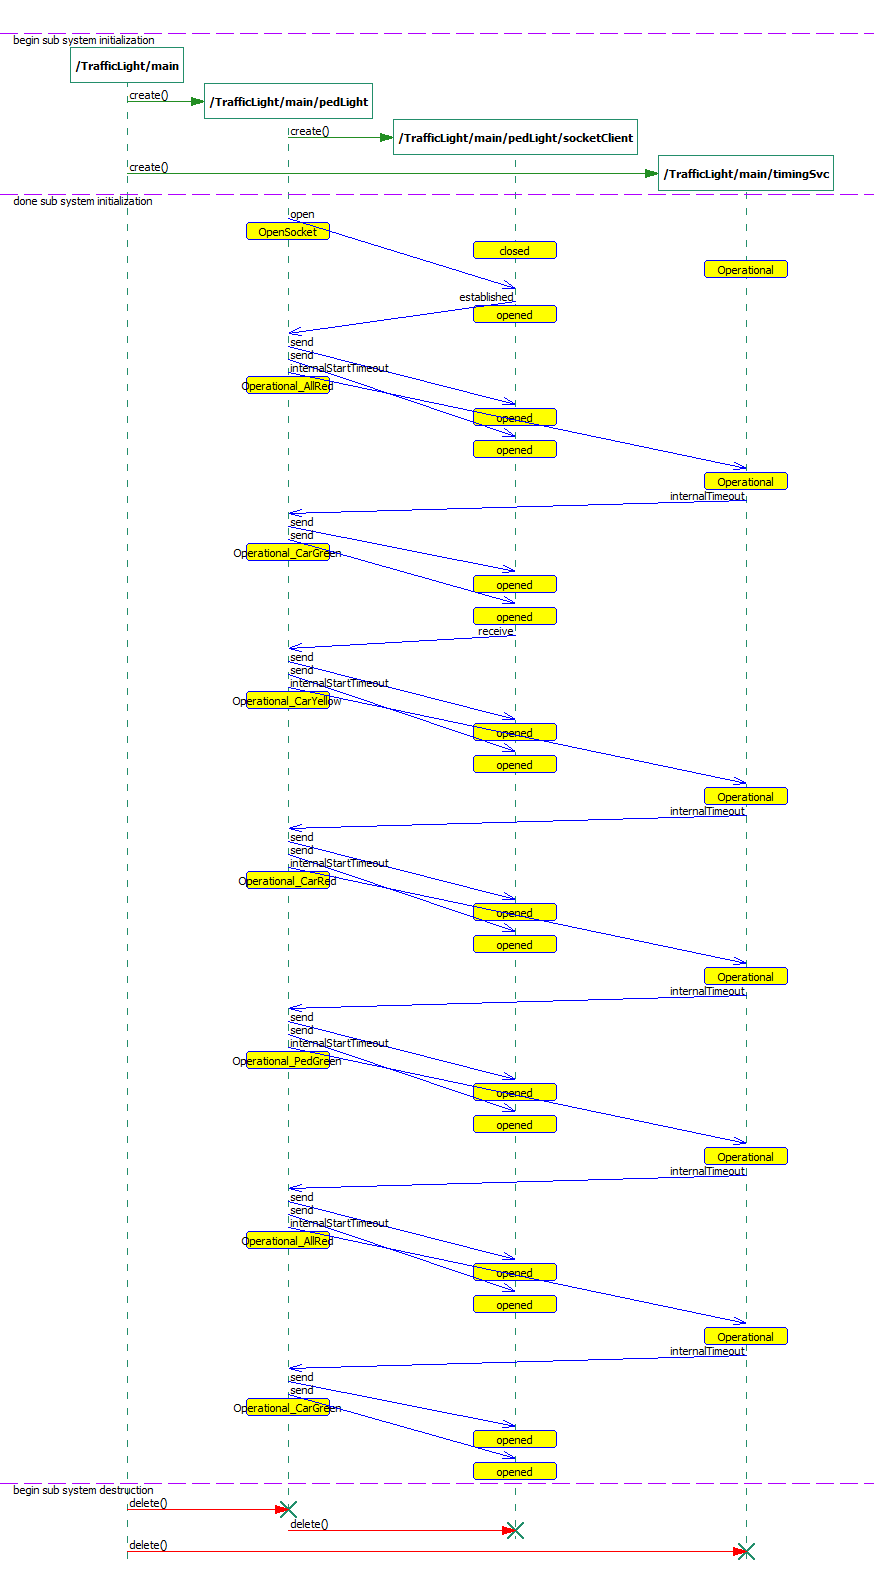
\includegraphics[width=0.8\textwidth]{images/018-msc.png}

\subsection{Configuration}

We want to use this example to illustrate how instance data can be configured using a configuration model.
We hard wired IP address and port into our model which of course is not very nice.

To use configurable data for our purpose we have to add a new attribute to out \textit{PedestrianLight} actor structure:

\begin{lstlisting}[language=ROOM]
Attribute ipConfig: DTcpControl [ "configuration of the IP-port for the communication with the Traffic Light GUI" ]
\end{lstlisting}

Then we add a configuration model to our \textit{model} folder.
The contents of this model has to be

\begin{lstlisting}[language=config]
ConfigModel TrafficLight {
	import TrafficLight.* from "TrafficLight.room"
	
	ActorInstanceConfig TrafficLight/main/pedLight {
		Attr ipConfig {
			Attr IPAddr="localhost"
			Attr TcpPort=4443
		}
	}
}
\end{lstlisting}

This way we can configure specific attributes of actor classes or instances.

Now we only have to add this model to our launch configuration for the generator, re-generate and we are done.

As an exercise to the reader we leave the following task. Add a second \textit{PedestrianLight} to the application and connect
it to a second GUI (listening on another port of course).

\subsection{The Complete Model}

As a reference here is the complete model:

\begin{lstlisting}[language=ROOM]
RoomModel TrafficLight {

	import room.basic.service.timing.* from "../../org.eclipse.etrice.modellib.java/model/TimingService.room"
	import room.basic.service.tcp.* from "../../org.eclipse.etrice.modellib.java/model/TcpService.room"
	import room.basic.types.* from "../../org.eclipse.etrice.modellib.java/model/Types.room"
	
	LogicalSystem TrafficLight {
		SubSystemRef main: Main
	}

	SubSystemClass Main {
		ActorRef pedLight: PedestrianLight
		ActorRef timingSvc: ATimingService
		LayerConnection ref pedLight satisfied_by timingSvc.timer
		LogicalThread defaultThread
	}

	ActorClass PedestrianLight {
		Structure {
			conjugated Port tcpControl: PTcpControl
			conjugated Port tcpPayload: PTcpPayload
			ActorRef socketClient: ATcpClient
			SAP timeout: PTimer
			Binding tcpControl and socketClient.ControlPort
			Binding tcpPayload and socketClient.PayloadPort
			Attribute ipConfig: DTcpControl [ "configuration of the IP-port for the communication with the Traffic Light GUI" ]
		}
		Behavior {
			Operation sendString(text: string) {
				"tcpPayload.send(new DTcpPayload(1, text.length(), text.getBytes()));"
			}
			Operation setLights(car: Light, ped: Light) {
				"sendString(\"carLights=\"+getCmd(car)+\"\\n\");"
				"sendString(\"pedLights=\"+getCmd(ped)+\"\\n\");"
			}
			Operation getCmd(light: Light): string {
				"switch(light) {
				case Light.RED: return \"red\";
				case Light.GREEN: return \"green\";
				case Light.YELLOW: return \"yellow\";
				default: return \"\";
				}"
			}
			StateMachine {
				Transition init: initial -> OpenSocket {
					action {
						"tcpControl.open(ipConfig);"
					}
				}
				Transition tr0: OpenSocket -> Operational {
					triggers {
						<established: tcpControl>
					}
				}
				State OpenSocket
				State Operational {
					subgraph {
						Transition init: initial -> AllRed { }
						Transition tr0: AllRed -> CarGreen {
							triggers {
								<timeout: timeout>
							}
						}
						Transition tr1: CarGreen -> CarYellow {
							triggers {
								<receive: tcpPayload>
							}
						}
						Transition tr2: CarYellow -> CarRed {
							triggers {
								<timeout: timeout>
							}
						}
						Transition tr3: CarRed -> PedGreen {
							triggers {
								<timeout: timeout>
							}
						}
						Transition tr4: PedGreen -> AllRed {
							triggers {
								<timeout: timeout>
							}
						}
						State AllRed {
							entry {
								"setLights(Light.RED, Light.RED);"
								"timeout.startTimeout(1000);"
							}
						}
						State CarGreen {
							entry {
								"setLights(Light.GREEN, Light.RED);"
							}
						}
						State CarYellow {
							entry {
								"setLights(Light.YELLOW, Light.RED);"
								"timeout.startTimeout(1000);"
							}
						}
						State CarRed {
							entry {
								"setLights(Light.RED, Light.RED);"
								"timeout.startTimeout(1000);"
							}
						}
						State PedGreen {
							entry {
								"setLights(Light.RED, Light.GREEN);"
								"timeout.startTimeout(3000);"
							}
						}
					}
				}
			}
		}
	}
	
	Enumeration Light {
		RED,
		GREEN,
		YELLOW
	}

}
\end{lstlisting}
